\documentclass[a4paper]{article} 
\usepackage{amsmath,amsfonts,amssymb,amsthm}
\usepackage{cite}
\usepackage{algorithmic}
\usepackage{graphicx}
\usepackage{subfigure}
\setlength{\parindent}{0cm}

\begin{document}
\title{Rectangle Graphs\\ for Genome Assembly}
\author{Nikolay Vyahhi, SP. and Pavel Pevzner}
\date{\today}
\maketitle

\abstract{The jigsaw puzzles were originally created by painting a picture on a 
flat rectangular piece of wood, and further, cutting that picture into
small pieces with a jigsaw.
The objective of any jigsaw puzzle is the rearragement of these pieces into a single structure with no gaps left between adjacent pieces. Additionally,
neighboring pieces must share an identical boundary as well as having similar color
and texture near the boundary.
While a general jigsaw puzzle is NP-complete, we introduce a simpler version of the jigsaw problem and
propose rectangle graphs for solving this problem in polynomial time. 
Interestingly, while usual applications of jigsaw problems are often limited to 
the assembly and repair of broken objects or 
the restoration of archeological findings, here we show that our simplified jigsaw puzzle
directly relates to the problem of assemblying genomes from mate-pairs. 
We implemented the rectangle graphs in  SPADES assembler and 
show that it out-performs other methods in both 
single-cell and multi-cell data. 
}

\newpage
\section{Introduction}

De Bruijn graphs have been used in many areas of bioinformatics, including genome assembly~\cite{Pevzner01},
repeats classification~\cite{Raphael04}, protein sequencing~\cite{Bandeira07},
and synteny blocks identification~\cite{Pham10}. In these applications, de Bruijn graphs are either constructed from a string or from a set of sub-strings of an
unknown string via gluing rules~\cite{Pham10,Raphael04}. 
In this work, we show that the idea of gluing rules for strings in de Bruijn graph can be
also adopted for multiple non-string objects, which can be used for the reconstruction of an object from
its broken pieces --- a general abstraction of the jigsaw puzzles. 


The jigsaw puzzles were originally created by painting a picture on a flat rectangular piece of wood, 
and further, cutting that picture into
small pieces with a jigsaw. The task of jigsaw puzzles requires the assembly of these small pieces into a valid picture with no gap or overlap between
them. Formally, the jigsaw problem can be defined as follow. Given a set $SP = \{ P_0, P_1,\ldots, P_n\}$ where $P_i$ represents the $i^{th}$ piece.
The objective of any jigsaw puzzles is the rearragement of these pieces into a single structure with no gaps left between adjacent pieces. Additionally,
neighboring pieces must share an identical boundary as well as having similar color and 
texture near the boundary.
Concrete applications of jigsaw puzzle solving are the assembly and repair of broken objects, 
or the restoration of archeological findings. Here we show
that the assembly problem from paired-end reads can also be formulated as a simple jigsaw problem.
In particular, in section 2, we describe a simple jigsaw puzzles and define rectangle graph to solve this 
problem, in section 3 we show the relation of the jigsaw puzzle to the 
problem of genome assembly using mate-pairs. In section 4, we describe how to adapt our approach 
to work with inexact insert size. Section 5 we apply our rectangle graph approach to 
assemble single cells as well as multiple cell datasets and demonstrate that it out-performs
other methods.

\section{A Simple Jigsaw Problem}



We consider a two-dimensional rectangular jigsaw puzzle created by the following procedure:
In stead of a complicated picture as it is usually the case for jigsaw puzzles, we simply draw a line $(d): y = x + D$ on a 2-$d$ coordinate Oxy.
On the vertical axis, define $n$ points: $A_1$, $A_2$, \ldots, $A_n$. On horizontal axis, define $m$ points
$B_1, B_2, \ldots, B_m$. The $m\times n$ combinations of these points defines a grid with $m\times n$ rectangles.  We further assign a label for each edge (there are
$m\times n$ edges) of the grid. The labeling of these edges is not unique, i.e., there may be different edges with the same label. We limit our attention to the
part of the grid that is intersected by the line and ignore all other parts (rectangles) that are not.
Given a value $D$,  the line $(d): y = x + D$ defines the \emph{diagonal grid graph} by retaining only the rectangles that are intersected by $(d)$.
In the classical sequence assembly problem, a fragment of the sequence is a substring. In this context, a \emph{fragment} is a
rectangle in the grid graph with a fragment of the line $(d)$ on it. For simplicity, we define the direction of each rectangle so that its orientation
is uniquely define in 2D space. Similar to the assembly problem where one attempts to reconstruct the genome from its
substrings, here we want to reconstruct the diagonal grid graph from individual rectangles.
An intuitive approach is to put the rectangles together such that their boundaries and diagonal lines match. Below, we formally define what constitutes
a valid solution for our simplified jigsaw version.

Given $n$ rectangles, each with a directed fragment of the line (d). We denote In(R): 
    the starting point of the fragment and Out(R): the ending point of
the fragment. The edges containing In(R) and Out(R) are called incoming surface and outgoing surface correspondingly. When In(R)/Out(R) coinsides with the
angle points of the rectangle, the surface becomes a single point.
Rectangle $R_1$ and $R_2$ are called neighbours if they share at least one vertex. Given two neighbouring rectangles $A$ and $B$, $A$ is
called extendable by $B$ ( or $B$ extends $A$) if the incoming surface of $B$ and the outgoing surface of $A$ as well as the locations of
the incoming and outgoing points are exactly aligned. Fig.~\ref{fig:basic} lists all 3 possible extensions of a given rectangle.
A figure is a valid solution to the jigsaw problem if every rectangle has one neighbor that extends it.
It is clear from the definition of the extension of pieces that a single line will be assembled from its multiple fragments on separated rectangles.
We are interested in the following problem.
\begin{figure}
\begin{center}
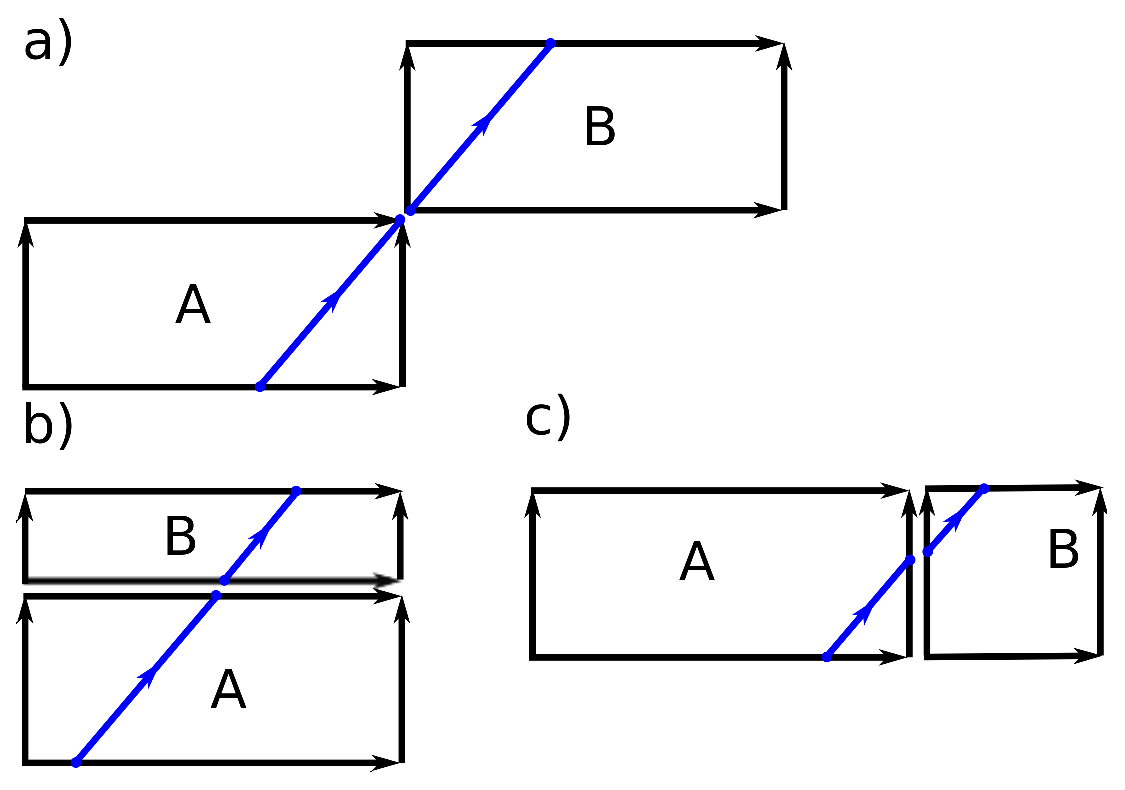
\includegraphics[scale=0.3]{fig/basic.eps}
\end{center}
\label{fig:basic}
\caption{Three possible extensions of rectangle $A$ based on its outgoing surface.}
\end{figure}

\textbf{Line Assemblying Puzzle}: \emph{Given $n$ rectangles generated by the described jigsaw generation procedure}
\begin{itemize}
\item \emph{Find the number of valid solutions.}
\item \emph{Enumerate all possible valid solutions.}
\end{itemize}

Below we define the rectangle graph which directly leads to solutions to this problem.

\textbf{Rectangle Graph:}
\begin{itemize}
\item  Define an initial graph $G_0$ on $2n$ vertices. For each rectangle $R$, introduce two new vertices $u$, $v$ and form an edge $u \rightarrow v$.
Label $u$ by the incomming surface and the position of the incoming point in the surface. Label $v$ by the outgoing surface and the position of the outgoing point
in the surface.
\item Glue vertices of $G_0$ together if they have the same label.
\end{itemize}

It is clear that each Eulerian tour in the rectangle graph corresponds to a valid solution of the jigsaw puzzle. The number of solutions is the number of
Eulerian tours in the graph, which can be characterized by the BEST \cite{best} theorem. The problem of enumerating all valid figures is reduced to the problem of enumerating
all Eulerian tours in the rectangle graph, a well studied problem \cite{abrham80}. 
Note that the original figure also corresponds to an Eulerian tour in this graph.  

%    \subsection{A General Fragment Assembly Problem}
%    A general fragment assembly problem tends to reconstruct the original \textbf{object} from its fragments. In particular, sequence fragment assembly tends to
%    reconstruct the original string from its substrings. Similarly, we can define the diagonal grid graph assembly problem from the set of all its rectangles. In particular,
%    given a set of rectangles, one approach to reconstruct the original diagonal grid graph is to align these fragments together such that the edges of adjacent rectangles
%    share the same label and the diagonal line can continue from one rectangle to its adjacent one.



\begin{figure}
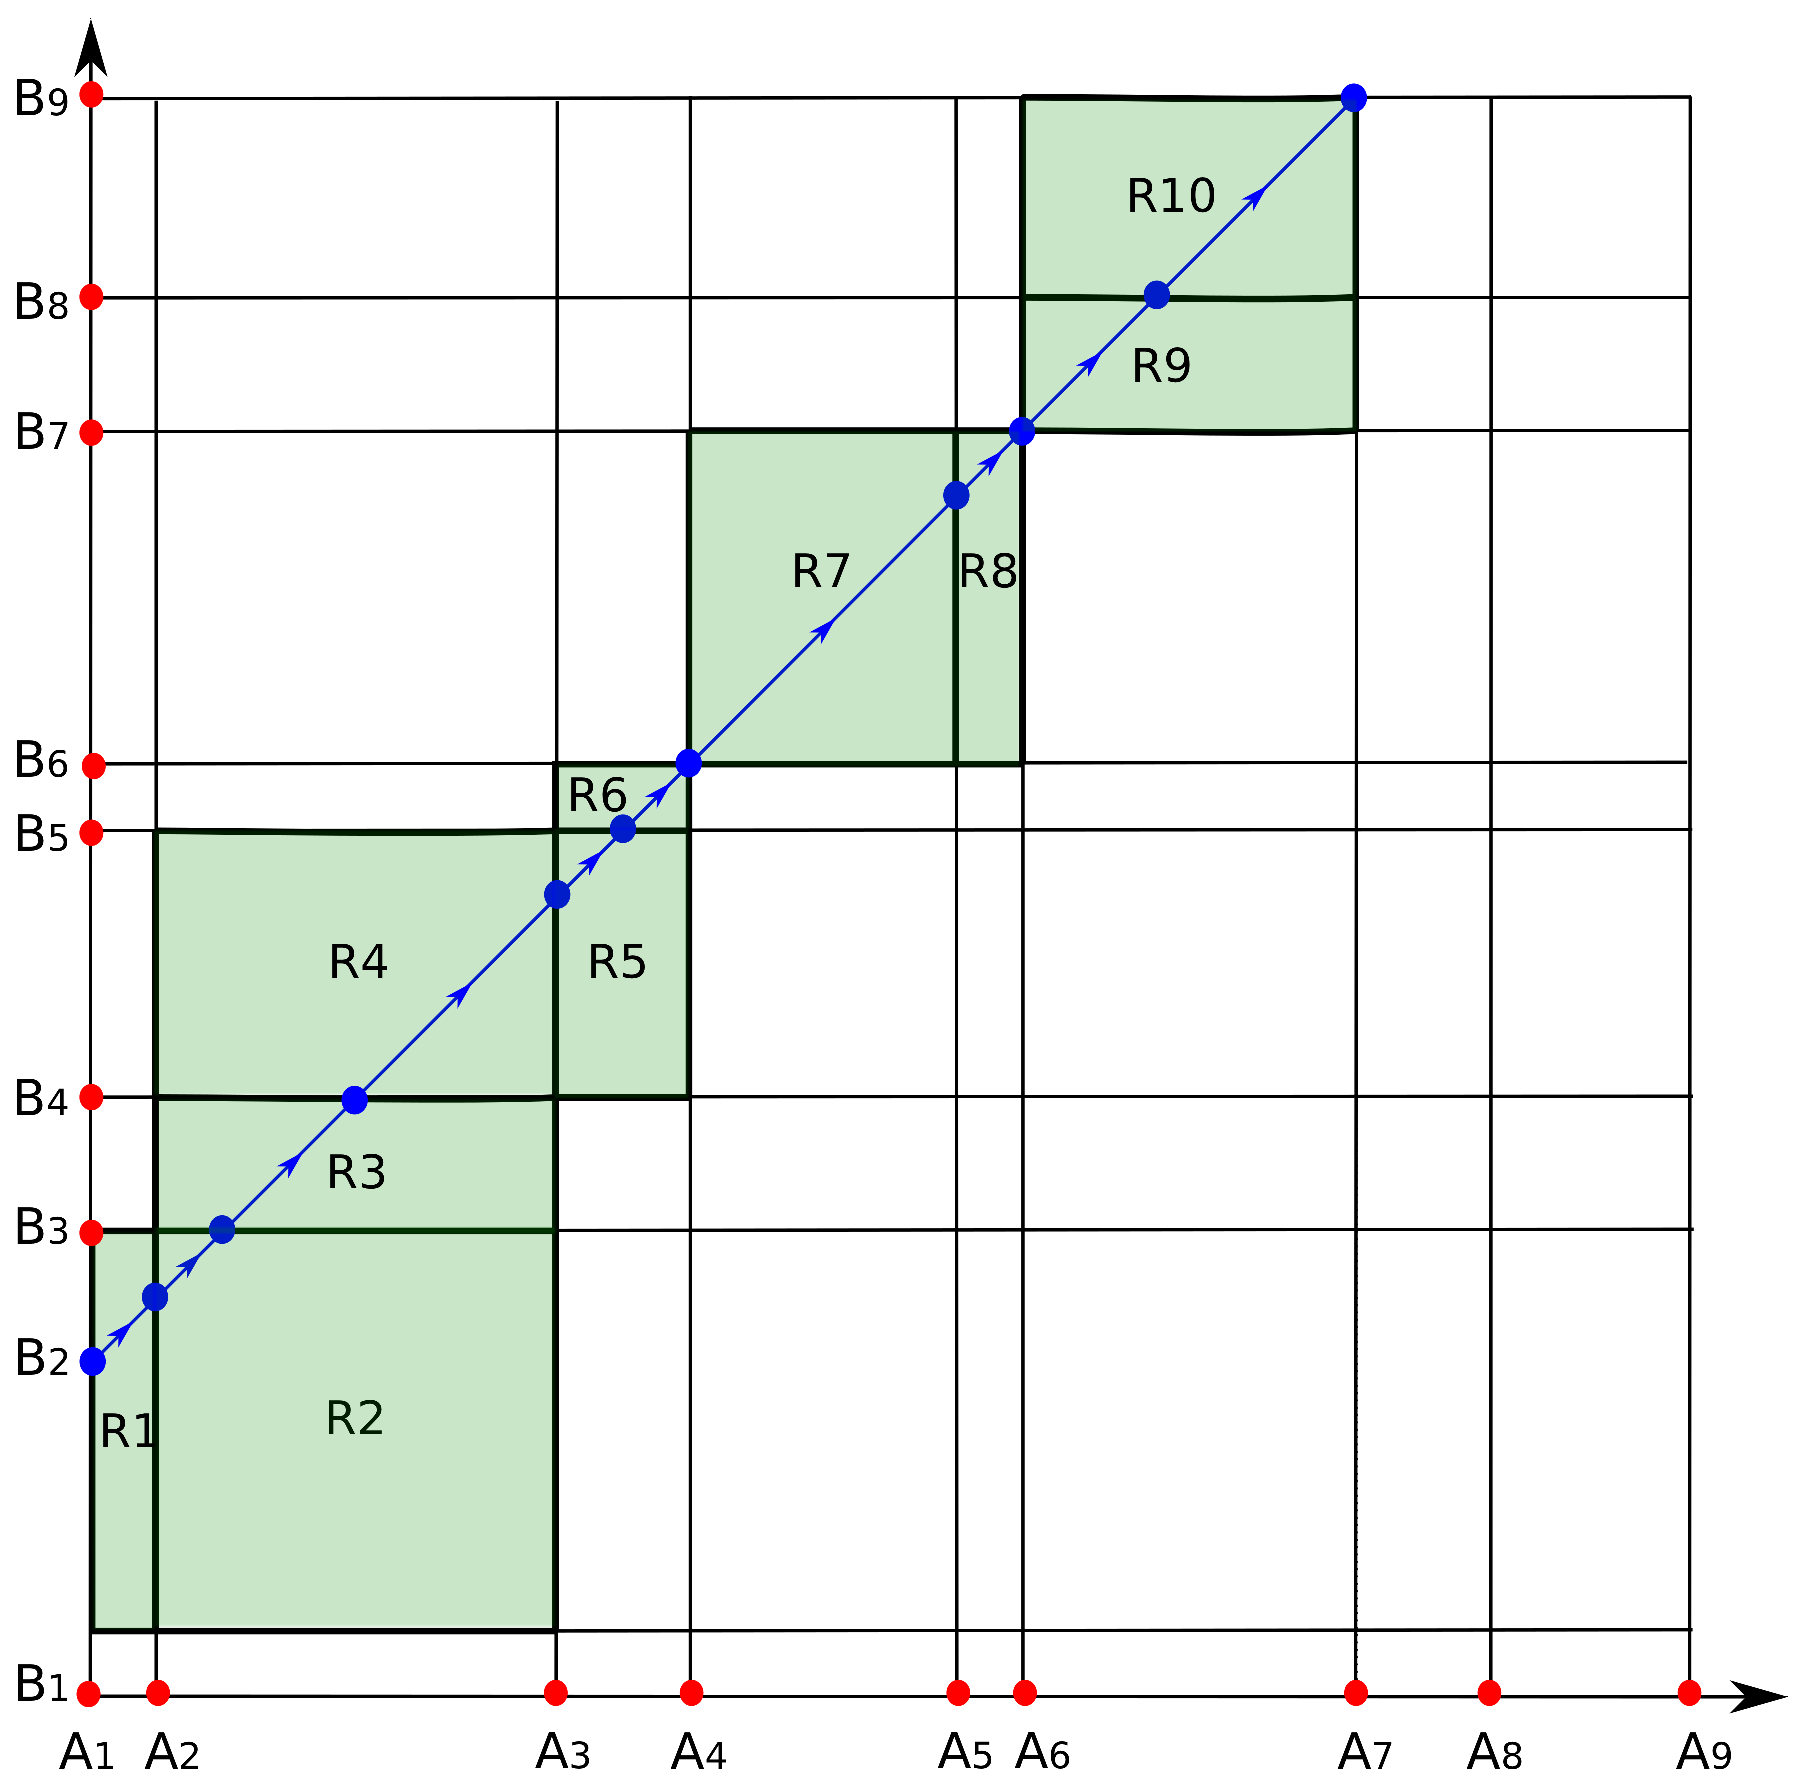
\includegraphics[scale=0.3]{fig/gridGraph.eps}
\caption{A sequence of $9$ points on horizontal axis and 9 points on horizontal axis forms a grid with $(9-1) \times (9-1)$ rectangles.
The diagonal grid graph (consists of blue rectangles --- rectangles intersected by the blue line). }
\end{figure}



\subsection{From Genome Assembly Using Mate-Pairs to Rectangle Graph}




We represent presented genomes as circular strings over the alphabet of nucleotides: $\{A,T,C,G\}$. 
A $k$-mer is a string of length $k$.
Given a $k$-mer $s = s_1\ldots s_k$,
we define $prefix(s)= s_1\ldots s_{k-1}$ and $suffix(s) = s_2\ldots s_k$. Given a multi-set $A$ of $k$-mers generated from a genome, 
the standard de Bruijn graph has directed edge $(prefix(s) \rightarrow suffix(s))$
for each $k$-mer $s\in A$.  A vertex $v$  precedes (follows) vertex $w$ if there exists an edge from $v$ to $w$ (from $w$ to $v$). The in degree ( out degree)  of a vertex 
$v$ is the number of vertices preceding (following) it.  A vertex $v$ is called a branching vertex if either its in degree or out degree is larger than 1. A path a $G$ is called a non-branching path if all of its vertices (except possibly the first and last) have indegree and outdegree
both equal to 1. These non-branching path represents contigs in the fragment assembly problem.


\noindent
\textbf{A 2D coordinate of the genome}
Alternatively, the genome can also be represented as a sequence of $(k-1)$-mers $a_1\ldots a_n$ where 
$a_i$ corresponds to a $k-1$-mer starting at position $i$ on the genome. 
Each element of $S$ also corresponds to a vertex in the de Bruijn graph $G$. 
Let $t$ be the number of $(k-1)$-mers in the genome that corresponds to the branching vertices in the
de Bruijn graph. The substring $a_i, \ldots a_j$ of $S$ connecting two consecutive branching 
vertices $a_i$ and $a_j$ corresponds to a non-branching path in the de Bruijn graph; we call 
$a_i\ldots a_j$ a non-branching substring of $S$.

We now form a 2D coordinate of the genome by representing the genome $S=a1\ldots a_n$ on
both vertical and horizontal axis. $t$ $(k-1)$-mers that correspond to the branching vertices 
in $G$ are colored in red in each axis. These points on both axis defines a grid, 
comprising of $t\times t$ rectangle. Each rectangle in this grid is defined by two adjacient branching 
vertices in vertical and two adjacient branching vertices in horizontal axis. 
Or equivalently, it is defined by a pair of (directed) non-branching substrings of $S$.    
In this coordinate, each point is labeled by a pair of $(k-1)$-mers. An edge of a rectangle is labeled 
by a list of all of its points.  

\noindent
\textbf{Mate-pairs and Diagonal Grid Graph}

Given a parameter $d$, a pair of $(k-1)$-mers $x$, $y$ forms a $(k,d)$-mer $(x|y)$  
of the genome $S = a_1\ldots a_n$ if there exists position $i$ such that $x=a_i$ and 
$y = a_{i+d}$ in $S$. The set of all $(k-1,d)$-mers of $S$ corresponds to a line $(d): y = x+d$. The 
line $(d)$ defines the \emph{diagonal grid graph} by retaining only the rectangles that 
are intersected by $(d)$. 

Below, we characterize the properties of the rectangles that are intersected by $(d)$. 
Since each rectangle $R$ is formed by a pair of non-branching substrings $\alpha = a_i\ldots a_{i+t1}$
and $\beta = a_i^*\ldots a_{i^*i+ t2}$, it is intersected by the line $(d)$ if and only if 
there exists $x$ such that $i\leq x \leq i+t1$ and $ i^* \leq x + d \leq i^* + t2$ (1). This condition
immediately leads to a property that there exists a $(k-1,d)$-mer $(a|b)$ of $S$ such that 
$a$ \emph{belongs} to $\alpha$ and $b$ \emph{belongs} to $\beta$.  A pair 
of non-branching substrings $\alpha$ and $\beta$ is called $d$-bounded if it corresponds to 
a rectangle intersected by $(d)$. The position where the (d) enters the rectangle is $(x^*,x^*+d)$ where 
$x^*$ is the minimum value  of $x$ such that condition (1) satisfies, and is labeled by 
a pair of $(k-1)$-mers $(a_x^*, a_{x^*+d})$.  The position where (d) exists 
the rectangle is $(\hat{x}, \hat{x+d})$ where $\hat{x}$ is the maximum value of $x$ such that the condition
(1) satisfies, and this position is labeled by a pair of $(k-1)$-mers $(a_{\hat{x}}, a_{\hat{x} +d})$


\noindent
\textbf{From mate-pair assembly with exact distance to the rectangle Graph}
While the line $(d)$ represents the 
set of points in the $2D$ coordinate (coordinate of pairs of $k$-mers), it uniquely defines the genome.
In the fragment assembly problem from a from a set of all $(k,d)$-mers of the genome, 
the diagonal grid graph is unknown, but each separated rectangle as well 
as the line segment on it can also be generated
from the set of $(k,d)$-mers. The task of assemblying the genome from mate-paired reads can be 
reduced to the problem of solving the simplified jig-saw problem from separated rectangles.
Below, we formally describe how separated rectangles can be constructed from mate-pair reads. 

\noindent
\textbf{Rectangle Graphs for inexact distance mate-pairs}



\section{Basics}

Given condensed de Bruijn Graph $G = <V,E>$ with $K$-mer vertices.
Length of edge $a$ is defined as number of $(K+1)$-mers in the edge. $\forall a: |a| \geq 1$.
Let $a_i$ be $i$-th $K$-mer in the edge $a$. $\forall a: 0 \leq i \leq |a|$
Let $d = insert\_size - reads\_length$ (called separation).
\section{Initial Set of Rectangles}
Define \textbf{rectangle} as ordered pair of edges $r = (a|b), \forall a, b \in E$.
Initially, we construct set of rectanges $R$ for all pairs of edges s.t. they contain at least one pair of $K$-mers within distance $d$ in graph $G$:
$$ R = \{ r | r = (a|b), \forall a, b \in E : \exists p = path(end(a), start(b)) : 0 \leq d - |p| \leq |a| + |b| \} $$

\section{What is Diagonal}

Define \textbf{point} in rectangle $(a|b)$ as ordered pair of $K$-mers in this edges $(a_i|b_j)$.

Define \textbf{d-point} as point $(a_i|b_j)$ s.t. distance between $a_i$ and $b_j$ in genome is $d$. The goal is to use all d-points and only, but we don't know the truth...

Two points are equal if their pairs of $K$-mers are equal.

Define \textbf{diagonal} $(a|b, D)$ in rectangle $(a|b)$ with offset $D$ s.t. $-|b| \leq D \leq |a|$ as list of points $(a_i, b_{i-D})$ for $i = max(D, 0) ... min(|a|, |b|+D)$.

Define \textbf{d-diagonal} as diagonal of only \textbf{d-points}. 

Length of diagonal is number of points in this diagonal. E.g. diagonal $(a|a, d)$ have length of $|a| - d + 1$.

Rectangles can contain multiple diagonals.

\section{Diagonal Support}

\textbf{Support} is our confidence that diagonal $(a|b, D)$ is actually d-diagonal.

Diagonal $(a|a, d)$ for long enough edge $a: |a| \geq d$ is always d-diagonal and doesn't require any other support.

Diagonal can be supported:
\begin{enumerate}
\item By points known to be d-points from the graph $G$, i.e. exists path of length $d$ (this initial support exists in all rectangles).
\item By points known to be d-points from paired reads. TODO: use insert size variation. TODO: use PHRED-quality of particular K-mers.
\item By points known to be d-points from single reads. E.g. if single read covers $a \rightarrow ... \rightarrow b$ connection and there exists rectangle $(a|b)$.
\item TODO: PathSets?
\item TODO: Neighbouring rectangles (diagonals) while gluing.
\item TODO: Other diagonals in the same rectangle (how? see section Gluing).
\end{enumerate}

Support of diagonal should scale by the length of diagonal.

\section{Rectangle Split}

The main goal is to filter and split rectangles, so that each rectangle contain d-diagonal and it is the only diagonal in this rectangle.

If one rectangle have multiple well-supported diagonals, we need to split it to multiple rectangles (one diagonal to each). Same applies for number of average-supported diagonals within variation (e.g. insert size variation), so their join is well-supported.

\section{Do we need rectangles?}

We can define everything only with diagonals, but it's simpler to draw them within rectangles.

Rectangle is equal to set (cluster) of diagonals. Rectangles splitting is somewhat similar to the current distance estimation.

\section{Diagonals Ranking}

We sort diagonals by their support. Better supported goes first.

\section{Diagonals Gluing}

We glue diagonals by their end-points only if this end-points are equal.

We glue diagonals in the order of their support:
\begin{itemize}
\item First we glue all well-supported diagonals (because they are d-diagonals).
\item We iterate over average-supported diagonals in the order of their support:
\begin{itemize}
\item If diagonal can connect two hanging end-points of already used diagonals, we glue it (preferable).
\item If diagonal can be glued to one hanging end-point of already used diagonal, we glue it.
\end{itemize}
\item We don't use poorly-supported diagonals.
\end{itemize}

\section{Gluing Support}

Original gluing support (rule) is equality of glued end-points of diagonals.

We can think about more gluing supports, e.g.:
\begin{enumerate}
\item Glue diagonals $(a|b, \cdot)$ and $(a|c, \cdot)$ only if there exists single read with $(K+2)$-mer which covers $b \rightarrow c$ path in graph. It's more powerful then single-read support for diagonals. TODO: $K+10$? $K+x$?
\item PathSets were supposed to be one of gluing supports --- glue two diagonals only if first's pathset is a prefix of second's pathset. We can somehow use PathSets also in the diagonal support, but I don't know how :)
\item TODO: more.
\end{enumerate}

\bibliographystyle{plain}
\bibliography{mybib}

\end{document}
